\chapter{The Hydrogen Atom}
In classical mechanics, the Hamiltonian $H$ for two bodies interacting via a - time independent- potential is given by :
\begin{equation}
(H= \sum_{i=1} ^2 \frac{(p_i)^2}{2 \mu}+ V(r)
\label{hamiltonian_1}
\end{equation}
Where, $ \mu = \frac{M+m}{Mm}$ is the reduced mass, and $r$ is the radial separation between the bodies. $p_i$ is the canonical momentum, that we may decompose into two parts :
\begin{align}
p_r =& \text{linear momentum} & p_t=& \frac{L}{r}\;\;\; \text{ angular momentum}
\end{align}
Hence, we may write \eqref{hamiltonian_1} as :
\begin{equation}
H = \frac{p^2}{2 \mu}+ \frac{L^2}{2\mu r^2} + V(r)
\end{equation}
since we know that the moment of inertia $I = \mu r^2$ we can therefore write: \marginpar{ recall that $L= I \omega$}
\begin{equation}
H = \frac{p^2}{2 \mu}+ \frac{L^2}{2I} + V(r)
\end{equation}
The potential for the Hydrogen atom is the Coulomb potential, given by the formula:
\begin{equation}
V(r) = - \frac{k e^2}{r}
\end{equation}
Hence we write the Hamiltonian function as :
\begin{equation}
H(p,r) =  \frac{p^2}{2 \mu}+ \frac{L^2}{2\mu r^2} - \frac{k e^2}{r}
\label{hafun}
\end{equation}
\section{Canonical quantisation of the H-atom  Hamiltonian }
We have the state $ | \Psi\rangle$ of the H-atom. We the define the Hamiltonian operator $ \hat H$ from quantising the Hamiltonian function in \eqref{hafun} that is :
\begin{equation}
\hat H = \frac{\hat p^2}{2 \mu}+ \frac{\hat L^2}{2\mu \hat r^2} - \frac{k e^2}{\hat r}
\label{haop}
\end{equation}
Due to the spherical symmetry, it is logical to project the state $ | \Psi\rangle$  into the configuration space in spherical polar coordinates, hereby the the Hilbert space is :
\[
\mathcal{H} : ( \mathcal{L} , d\mu)
\]
where $ d\mu = dr\;d^2 d\phi \; \sin\phi ^2 d\theta$ , the volume element in the spherical polar coordinates and the wavefunction:
\[
\psi (r, \phi, \theta) = \langle r, \phi,\theta | \psi \rangle
\]
The H-atom is surely a stationary state $ \Psi(r, \phi, \theta;t) = \psi (r, \phi, \theta) e^{ -i\omega t}$.Hence the time-independent Schr\"{o}dinger's equation is written as :
\begin{equation}
-\frac{\hbar ^2}{2 \mu} \nabla^2 \psi (r, \phi, \theta) - \frac{k e^2}{r} \psi (r, \phi, \theta) = E \psi (r, \phi, \theta)
\label{TISE}
\end{equation}
It was found -mathematically- that the wavefunction can be separated into three parts:
\begin{equation}
\psi (r, \phi, \theta) = R(r) P(\phi)F(\theta)
\end{equation}
Where $R(r)$ is the radial function, and $ P(\phi)F(\theta)$ make up the spherical Harmonics $ Y(\phi,\theta)$.
\section{Quantum numbers}
Each of the functions above is an eigenfunction for some observable about the hydrogen atom with an associated quantum number:
\begin{align*}
R(r) &\longrightarrow n = 1,2,3 \dots\; \; \; \; \; \; \;  \text{Principle quantum number } \\
F(\theta)&\longrightarrow  \ell= 0,1,2\dots, n-1 \; \; \; \; \; \; \;  \text{orbital quantum number } \\
P(\phi)&\longrightarrow m_ \ell= -\ell, -\ell+1,\dots,+\ell \; \; \; \; \; \; \;  \text{megnatic quantum number } 
\end{align*}
\section{Solution of the TISE for the Hydrogen}
In fact, the H-atom is the only physical problem in quantum mechanics that can be solved exactly without using perturbation theory or other approximation methods. The TISE \eqref{TISE} can written as three differential equations:
\begin{subequations}
	\begin{align}
	\frac{1}{R(r)} \frac{d}{dr}\left( r^2\frac{d R(r)}{dr}\right) +\frac{2\mu}{\hbar ^2}\left( Er^2+k e^2\right)  &= \ell(\ell+1)\\
	\frac{\sin \theta}{F(\theta)} \frac{d}{d \theta} \left( \sin \theta \frac{d F( \theta)}{d \theta}\right) + C_r \sin^2\theta &= - C_\phi \\
	\frac{1}{P(\phi)} \frac{d^2 P(\phi)}{d \phi ^2}&= C_\phi
	\end{align}
\end{subequations}
Solving the above equations to obtain the full expression for the wavefunction:
\begin{equation}
\boxed{
	\psi_{ n, \ell, m_ell}(r, \phi, \theta) = A_{r \ell} \, e^{-r/a_0 r}\; r^\ell L _{n \ell} ( \frac{r}{a_0}) \cdot Y ^\ell_m ( \phi, \theta) }
\label{h-atom}
\end{equation}
Where:
\begin{itemize}
	\item $A_{r \ell}$ , a normalisation constant.
	\item $a_0$, Bohr radius and it is equal to $ \approx0.53 \AA$.
	\item $L _{n \ell} ( \frac{r}{a_0})$, the associated Laguerre polynomial.  
	\item $Y ^\ell_m ( \phi, \theta)$, the associated spherical harmonics, the eigenfunction for the operators $ \hat L$ and $\hat L_z$. 
\end{itemize}
We can find the energy spectrum for the Hydrogen atom from \ref{h-atom} :
\begin{equation}
\boxed{E_n = -\left(\frac{\mu\, e^2 }{8 \epsilon_o ^2 \hbar^2}\right)  \frac{1}{n^2} \; \; \; = - \frac{13.6 \; eV}{n ^2}}
\end{equation}
With $ \epsilon_o$ the vacuum permittivity. \\
As expected, the spectrum is discrete, but the spacing between the energy levels gets smaller and smaller as the principle quantum umber increases, figure \ref{fig_1} \\
\begin{figure}[h]
	\centering
	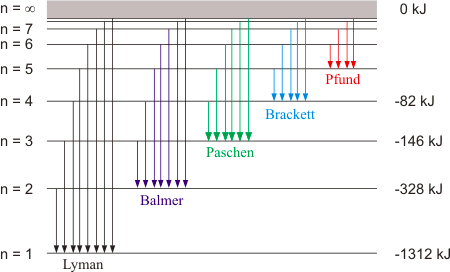
\includegraphics[scale =0.6]{./figures/levels}
	\label{fig_1}
	\caption{ Energy levels of the idealised H-atom and the well-known spectral series associated with electron transitions}
\end{figure}
If we wish to find the \textit{ionisation energy  }  for hydrogen atom ( i.e. the energy required to free the electron from the atom) we let $ n\rightarrow \infty$ we obtain:
\[
E_\infty = 13.606 \; eV = Ry
\]
it is equal to the Rydberg energy .  For generality we can approximate the energy spectrum for any atom having $Z$ electrons and $ \mu$ reduced mass by:
\begin{equation}
E \sim -Z^2 \frac{\mu}{m_e}Ry
\end{equation}
We ought to emphasise this is merely a hand-waving approximation ! The true energy spectrum for atoms ( even the H-atom)  is far more complicated, as we shall see later when we study the Real Hydrogen atom.
\section{Degeneracies in the ideal H-atom}
Since \eqref{h-atom} depends on three quantum numbers $ , \ell$ and $ m_\ell$, but the energy spectrum only depends on $n$, we have \textit{degenerate states} in the idealised H-atom. Where we can have multiple wavefunctions having the same energy. For example, in the first excited state $ n=2$ we have the following wavefunctions:
\[
\psi_{2,0,0} \; \; \; \psi_{2,1,0}  \; \; \; \psi_{2,1,-1}  \;\; \psi_{2,1,1} ,
\]  
and so on .
However, the number of electrons that can occupy each energy level is determined by \textbf{Pauli exclusion principle:} stating that no two electrons in the atom can wave an overlapping wavefunctions. In other words each wavefunction can describe one electron only. Meaning no electrons in the atom can have all of their quantum numbers identical. 
\section{ Spin quantum number}
In addition to the quantum numbers $( n, \ell, m_\ell)$ there is a forth quantum number of the electron, corresponding to its \textbf{spin}, which is an internal degree of freedom electrons are found to possess. The spin quantum number $ m_s$ can take one of two values $ \pm \frac{1}{2}$ of multiples of $\hbar$. So far, this new quantum number does not seem to affect the energy spectrum. However, we shall see later that it player a r\"{o}le in an interaction inside the H-atom affecting the energy spectrum.
\section{Problems}
\begin{enumerate}
	\item If you know that the ground state radial function of the H-atom is given by:
	\[ R_{10}= e^{-r/a_0}\]
	\begin{enumerate}
		\item Normalize it .
		\item Construct $\psi_{100}$.
		\item Calculate $\langle r \rangle$ , $ \langle r^2\rangle, \langle x\rangle $ and $\langle x^2\rangle$, what do you observe?  
	\end{enumerate}
	\item Derive the Rydberg formula for the H-atom. Then obtain similar formulas for D-atom and positronium (electron orbiting its anti particle) .
	\item Having Pauli exclusion principle in mind, what is the maximum number of electrons one can have in each shell ( for a given $n$ ) ?
	\item The H-atom  emission spectrum is observed to be described in the picture below
	\begin{figure}[h!]
		\centering
		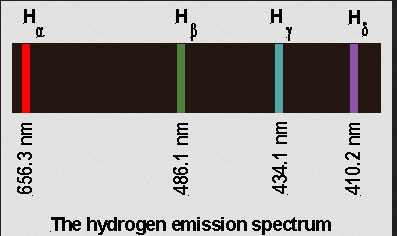
\includegraphics[scale=0.6]{./figures/spectrum}
	\end{figure}
	\begin{enumerate}
		\item If there is only one electron in the H-atom, how do you explain the existence of multiple emission lines ?
		\item Explain the spectrum in detail, using the Rydberg formula.
		\item Spectroscopy is used to distinguish between the isotopes of elements ( $H_2$ and $ D_2$ for example). Predict the $D_2$ spectrum and draw it, compare it the given $H_2$ spectrum.
	\end{enumerate}
	\item Compare the energy spectrum of the H-atom, with the one in a 3-D box of dimension  $1$ \AA . 
	\item Show that:
	\[ \langle \frac{\partial U}{\partial r}\rangle = \langle \frac{1}{r^2}\rangle\]
	If $U$ is the Coulomb potential.
	\item Is it possible for electrons to exist in the nucleus ?
	Justify your answer using the calculation of probability for the electron to be detected within the nuclear radius $ r_{nuclear} \sim^{-15}$ m.
	\begin{enumerate}
		\item Start by using the wavefunction $ \psi_{100}$, and show it is valid for all values of$r$ up to $r=0$.
		\item Assume that the wavefunction is constant over the small volume of the `spherical nucleus' then calculate the probability $ P \approx V_{nuclus} \times | \psi_{100}|^2$.
		\item The previous step can be done in more `sophisticate way' by expanding the wavefunction around the origin using the parameter $ \epsilon = 2r_{nuclear}/a$
		\item substitute for $a_0$ and $r_{nuclear}$ to estimate the probability.
	\end{enumerate}
	\item The associated Laguerre polynomials are given by the following  ` generating formula ':
	\[ L(x) ^P_ {q-p} = (-1)^p \left( \frac{d}{dx}\right) ^p L_{q}\]
	With $L(x)_a$ is the Laguerre polynomials give by:
	\[ L(x)_q = e^{x}\left( \frac{d}{dx}\right)^q (e^{-x}x^q)\]
	Use these equations to generate the first two associated polynomials.
	Are they orthonormal over the interval $ [ 0, + \infty]$ and weighting function $ w(x) = x^p e^{-x}$ ?
\end{enumerate}